%\documentstyle[aas2pp4,epsf]{article}
%%%\documentstyle[aaspp4,epsf]{article}
%\documentstyle[12pt,aasms]{article}    % this is for a preprint
%(single-spaced)
%\documentstyle[aaspp4,epsf]{article} % this is for small print
%\documentstyle[12pt, aaspp4]{article}

%\documentstyle[11pt,aaspp]{article}
%\documentclass[12pt, preprint]{aastex} 

\documentclass[manuscript]{aastex}
%\documentclass[apj]{emulateapj}

%\documentclass[12pt, preprint,numberedappendix]{emulateapj}
%\documentstyle[12pt,aasms]{article}    % this is for submittal
                                       % (double-spaced)

%\documentstyle[12pt,aasms]{article}   \usepackage{emulateapj5} 

\usepackage{graphicx} 
\usepackage{amsmath}
\usepackage{hyperref}
\usepackage{amsfonts}
\usepackage{amsmath}
\usepackage{amssymb}
\usepackage{amsthm}
\usepackage{subeqnarray}
\usepackage{ulem}
%\bibliographystyle{apj}

\newcommand{\delad}{\nabla_{\rm ad}}
\newcommand{\delrad}{\nabla_{\rm rad}}
\newcommand{\emgr}[1]{\emph{ \color{gray} #1}}

\newcommand{\ie}{i.e.\ }
\newcommand{\eg}{e.g.\ }
\newcommand{\p}{\partial}
\newcommand{\xv}{\vc{x}}
\newcommand{\kv}{\vc{k}}
\newcommand{\brak}[1]{\langle #1\rangle}


\newcommand{\gcc}{\;\mathrm{g\; cm^{-3}}}
\newcommand{\gsc}{\;\mathrm{g\; cm^{-2}}}
\newcommand{\cm}{\; {\rm cm}}
\newcommand{\mm}{\; {\rm mm}}
%\newcommand{\ps}{\; {\rm s^{-1}}}
\newcommand{\km}{\; {\rm km}}
%\newcommand{\au}{\; \varpi_{\rm AU}}

\newcommand{\AU}{\; {\rm AU}}
\newcommand{\yr}{\; {\rm yr}}
\def\K{\; {\rm K}}

\newcommand{\vcs}[1]{\mbox{\boldmath{$\scriptstyle{#1}$}}}
\newcommand{\vc}[1]{\mbox{\boldmath{$#1$}}}
\newcommand{\nab}{\vc{\nabla}}
\DeclareMathSymbol{\varOmega}{\mathord}{letters}{"0A}
\DeclareMathSymbol{\varSigma}{\mathord}{letters}{"06}
\DeclareMathSymbol{\varPsi}{\mathord}{letters}{"09}

\newcommand{\Eq}[1]{Equation\,(\ref{#1})}
\newcommand{\Eqs}[2]{Equations (\ref{#1}) and~(\ref{#2})}
\newcommand{\Eqss}[2]{Equations (\ref{#1})--(\ref{#2})}
\newcommand{\Eqsss}[3]{Equations (\ref{#1}), (\ref{#2}) and~(\ref{#3})}
\newcommand{\App}[1]{Appendix~\ref{#1}}
\newcommand{\Sec}[1]{Sect.~\ref{#1}}
\newcommand{\Chap}[1]{Chapter~\ref{#1}}
\newcommand{\Fig}[1]{Fig.~\ref{#1}}
\newcommand{\Figs}[2]{Figs.~\ref{#1} and \ref{#2}}
\newcommand{\Figss}[2]{Figs.~\ref{#1}--\ref{#2}} 
\newcommand{\Tab}[1]{Table \ref{#1}}

\newenvironment{packed_item}{
\begin{itemize}
  \setlength{\itemsep}{1pt}
  \setlength{\parskip}{0pt}
  \setlength{\parsep}{0pt}
}{\end{itemize}}

%\newcommand{\delad}{\nabla_{\rm ad}}
%\newcommand{\delrad}{\nabla_{\rm rad}}
\newcommand{\Rg}{\mathcal{R}}
\newcommand{\RB}{R_{\rm B}}
\newcommand{\co}{_{\rm c}}
\newcommand{\di}{_{\rm d}}
\newcommand{\cb}{_{\rm RCB}}
\newcommand{\surf}{_M}
\newcommand{\mc}{m_{\rm c \oplus}}
\newcommand{\mcn}[1] { m_{ \rm c #1 \oplus} }
\newcommand{\MC}{M_{\rm crit}}
\newcommand{\au}{a_\oplus}
\newcommand{\aun}[1]{ a_{#1\oplus} }

\begin{document}
\bibliographystyle{apj}

\title{The role of disk volatile chemistry and dynamics in shaping the compositions of nascent planets}
\author{Ana-Maria A. Piso}
\affil{Advisor: Karin I. \"Oberg}
\affil{Suggested Thesis Advisory Committee members: \\ Dimitar Sasselov, Sean Andrews, Matthew Holman}

\section{Introduction and Motivation}



The chemical composition of giant planet atmospheres can provide important constraints on the formation of these planets, as well as on their accretion and migration history. 



An important signature of atmospheric chemistry in giant planets is the C/O ratio. The C/O ratio has been estimated observationally in some giant planets, and it has been found to be different than the solar C/O ratio of the host star \citep{madhu11}. One explanation for this difference was proposed by \citet{oberg11}. Their basic idea was that the main carriers of carbon and oxygen, i.e. H$_2$O, CO$_2$ and CO, have different condensation temperatures. This results in variations in the abundances of C and O in solids and gas between the snow lines of the volatiles mentioned above. Figure \ref{fig:CtoO} shows the C/O ratios in the gas and in the dust as a function of semimajor axis, for a passively irradiated disk. %As a fiducial disk model we choose the prescription of \citet{chiang10} for the gas temperature and surface density profile:

%\begin{eqnarray}
%\label{eq:diskmodel}
%T_{\rm d} = 120 \times (a/\rm AU)^{-3/7} \,\,\, \rm K \\
%\Sigma_{\rm d} = 2000 \times (a/\rm AU)^{-1} \,\,\, \rm{g \, cm}^{-2},
%\end{eqnarray}
%where $a$ is the semimajor axis.


\begin{figure}[htb]
\centering
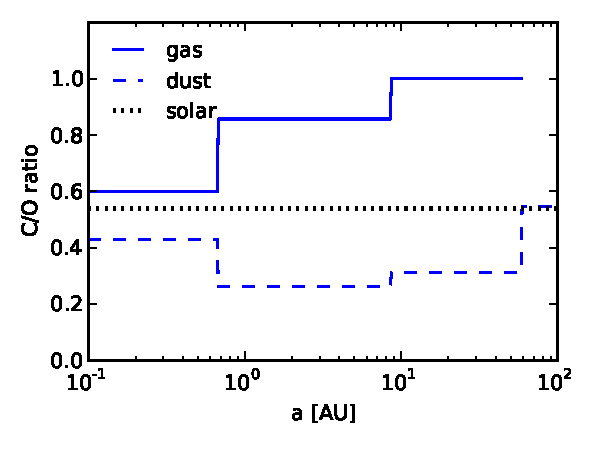
\includegraphics[width=0.8\textwidth]{../figs/C_O_ratio_2.pdf}
%\vspace{-0.5in}
\caption{C/O ratio in gas and in dust as a function of distance, for a passively irradiated protoplanetary disk. After \citet{oberg11}.} %  (See text for a description of evolution to yet higher masses.) 
\label{fig:CtoO}
\end{figure}

The relative abundance of C and O in gas and dust across the protoplanetary disk is further affected by various chemical and dynamical process occurring in the disk throughout its lifetime. The chemical composition and distribution of the main C and O carriers evolves with time (e.g., \citealt{ciesla06}, \citealt{visser09}), as do the location and shape of the different snowlines (e.g., \citealt{garaud07}, \citealt{stevenson88}). Moreover, solids are redistributed throughout the protoplanetary disk due to radial drift \citep{chiang10} and planetary migration \citep{armitage10}. Observations have shown that young Sun-like stars actively accrete gas from the disk (e.g., \citealt{hartmann06}), which may further change the abundance of volatiles in solid and gaseous form in the disk. Exploring and quantifying the effect of all such processes on the atmospheric composition of giant planets is crucial for our understanding of their formation and overall evolution in the protoplanetary disk. 

\section{Proposed Research}

In this thesis, I plan to investigate the various chemical and dynamical processes that take place in protoplanetary disks, and understand which of these processes are relevant for the chemical variations in the atmospheres of gas giants, and under which conditions. I aim to enhance the toy model of \citet{oberg11} by including dynamical effects, as well as a more complex chemical reaction network. The physical processes that I will consider, as well as the timeline of my thesis, can be summarized as follows. 

\subsection{Radial Drift of Solids}
\label{sec:drift}

Solid planetesimals in disks orbit their host star at a Keplerian velocity. The gas, on the other hand, experiences an extra pressure gradient, which causes it to rotate at a sub-Keplerian velocity. Thus solid particles experience a headwind, which tends to remove angular momentum and cause the planetesimals to spiral inwards and fall into the host star. Small planetesimals are well-coupled to the gas, so they rotate with the gas at the sub-Keplerian frequency and their drift timescales are very large compared to the lifetime of the gas disk. Conversely, large planetesimals are decoupled from the gas, thus the influence of gas drag on them is negligible and their radial drift times also exceed the disk lifetime. On the other hand, planetesimals of intermediate sizes ($\sim$0.1cm - $\sim$10 km, depending on their location and the disk temperature and surface density profile) can have short drift timescales relative to the disk lifetime. If  the drift timescale is shorter than the evaporation timescale, planetesimals might drift a significant distance past a given snowline before they desorb. This therefore changes the location and shape of snowlines, and thus the C/O ratio from the profile depicted in Figure \ref{fig:CtoO}.

The calculation of \citet{oberg11} assumes a passively irradiated disk. However, observations have shown that young Sun-like stars actively accrete gas from the disk at typical rates $\dot{M}_{\rm gas} \sim 10^{-8}$ $M_{\odot}$/year (e.g., \citealt{hartmann06}). The abundance of H$_2$O, CO$_2$ and CO in gas and grains, and therefore the C/O ratio in gas, will depend on the relative mass accretion rates of solids (due to drift) and of gas (due to viscosity). The surface density of planetesimals (and thus the C/O ratio) is further affected by grain growth and particle fragmentation (e.g., \citealt{birnstiel12}).

I will incorporate the effect of radial drift, particle growth and gas accretion, coupled with the desorption of ices, to calculate the C/O variation with semimajor axis in an actively accreting protoplanetary disk. \textbf{This will result in Paper I, estimated completion spring 2015}.

\subsection{Nitrogen Abundance}
\label{sec:nitrogen}

Besides carbon and oxygen, nitrogen is another important volatile molecule that shapes the chemistry in protoplanetary disks. Nitrogen is primarily found as $\rm{N}_2$, although $\sim$$10$\% of the disk nitrogen abundance can be carried by $\rm{NH}_3$ (e.g., \citealt{lahuis00}). I plan to add nitrogen to the simple chemical model of section \ref{sec:drift} and apply the model summarized in section \ref{sec:drift} to study the effect of radial drift on the N/O ratio in protoplanetary disks. \textbf{This will result in Paper II, estimated completion summer 2015} \textit{(Is this too little content for just one paper? Perhaps this could be a letter?)}. 

\subsection{The Effect of Disk Chemistry on the Shape and Location of Snowlines}

The calculations summarized in sections \ref{sec:drift} and \ref{sec:nitrogen} are based on a simplified, static chemical model. In reality, however, the gas-grain chemical network in protoplanetary disks is complex and evolves with time (e.g., \citealt{bergin09}, \citealt{fogel11}). In this part of my thesis, I plan to incorporate the detailed, time-dependent chemical reaction network developed by Merchantz et al. (in prep.) \textbf{(?)} in the radial drift calculation described in section \ref{sec:drift}. \textbf{This will result in Paper III, estimated completion late 2015 / early 2016} \textit{(Too much content for one paper? Should it be split into (Paper III) just the effect of evolving disk chemistry on snowline location, and (Paper IV) chemistry + drift?)}.

\subsection{Dynamical Effects II: Core Accretion, Migration, Core Dredging}

In this part of the thesis, I plan to incorporate further dynamical effects, such as atmospheric pollution of planetesimals during the atmospheric accretion phase, Type I and Type II migration, and core dredging (e.g., \citealt{lodders09}, \citealt{stevenson85}, \citealt{guillot04}). \textbf{This will result in Paper IV, estimated completion summer 2016} \textit{(Again, perhaps too little material for one paper?)}.

\subsection{Potential Planet Formation Locations and Comparison with Observations}

In the last part of my thesis, I plan to analyze the results obtained in the previous sections, asses the relevance of each chemical or dynamical effect considered, and combine the relevant processes to obtain a realistic framework for analyzing the relation between atmospheric chemical composition and  formation history for a given planet. I will then use this framework to explore a wide parameter space of initial disk conditions in order to generate model planet populations and explore potential planet formation locations. By comparing my results with present and future observations of atmospheric spectra of giant planets, I will be able to further constrain their formation, accretion and migration history. \textbf{This will result in Paper V, estimated completion spring 2017.}

\section{Preliminary Results}

As a first step, I investigate the effect of radial drift on the shape of snowlines in protoplanetary disks (see section \ref{sec:drift}). I calculate self-consistently the drift and desorption distances as a function of particle size for a passively irradiated disk. I calculate the desorption rates following the prescription of \citet{hollenbach09}, assuming that the solids are perfect spheres and composed of a single volatile material (either H$_2$O, CO$_2$ or CO). To calculate the drift timescale, I follow the analytic prescription of \citet{chiang10}. I integrate the drift and desorption equations self-consistently, and stop the evolution at $\tau=3$ Myr, the typical lifetime of a protoplanetary disk. 

\begin{figure}[htb]
\centering
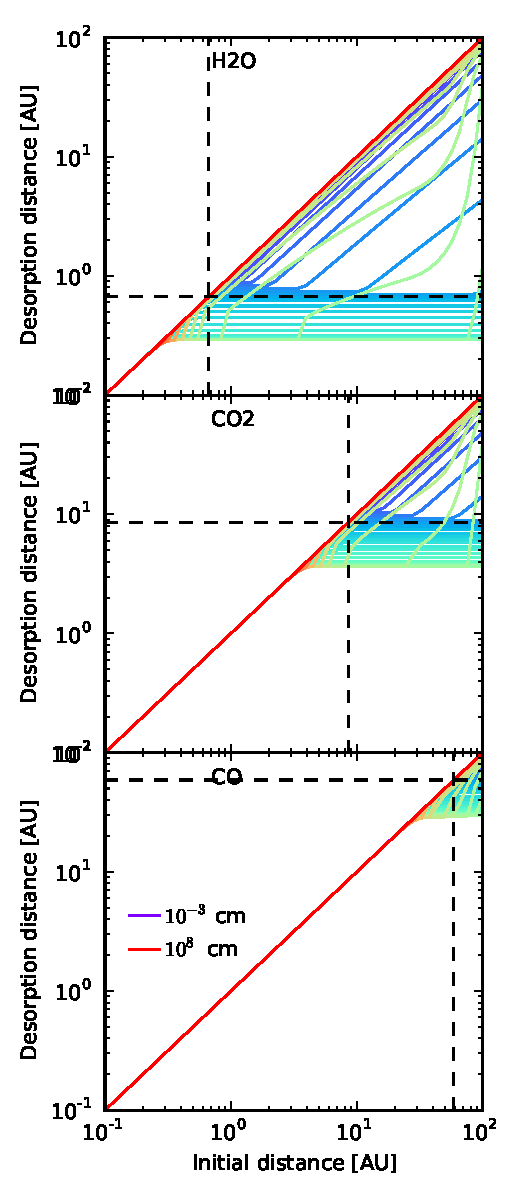
\includegraphics[width=0.47\textwidth]{../figs/desorption_distance_many_new_2.pdf}
%\vspace{-0.5in}
\caption{Desorption distance as a function on initial particle distance for H$_2$O (top panel), CO$_2$ (middle panel) and CO (bottom panel), for particle size between $10^{-3}$ and $10^8$ cm. The vertical and horizontal dashed lines show the respective snowlines as calculated based on \citet{hollenbach09}. Small particles desorb instantaneously, while large particles do not either drift or desorb before disk dissipation. Intermediate size planetesimals desorb at a fixed distance that depends on the particle size, regardless of their initial location in the disk.} %  (See text for a description of evolution to yet higher masses.) 
\label{fig:drift_dist}
\end{figure}

\begin{figure}[htb]
\centering
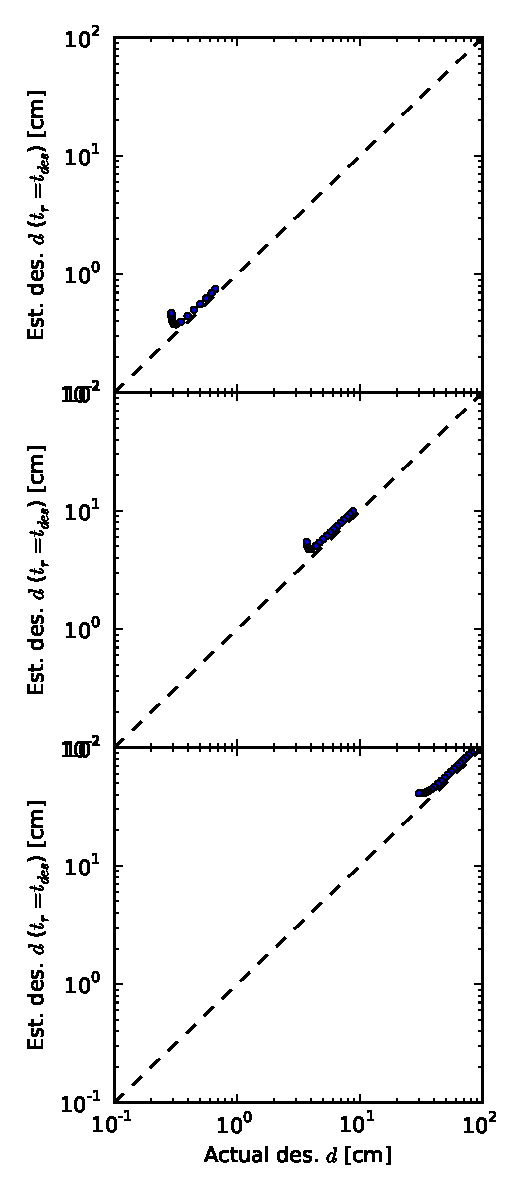
\includegraphics[width=0.5\textwidth]{../figs/desorption_distance_actual_vs_estimated.pdf}
%\vspace{-0.5in}
\caption{Desorption distance estimated analytically (when the drift and desorption times are equal) versus the desorption distance calculated numerically, for H$_2$O (top panel), CO$_2$ (middle panel) and CO (bottom panel), and for different initial particle sizes. The analytic and numerical results are in good agreement.} %  (See text for a description of evolution to yet higher masses.) 
\label{fig:an_vs_num}
\end{figure}

Figure \ref{fig:drift_dist} shows the desorption distance as a function of the initial planetesimal location, for H$_2$O, CO$_2$ and CO particles. As expected, small planetesimals desorb instantly, while large boulders do not have enough time to either desorb or drift before the disk dissipates. Notice, however, that planetesimals with sizes between $\sim 1$ cm and $\sim 10^3$ cm desorb at a fixed distance from the host star, regardless of their initial location in the disk. This desorption distance depends on the planetesimal size. I have found that this distance can be well approximated analytically as the radius at which the desorption and drift timescales are equal (see Figure \ref{fig:an_vs_num}). %Figure \ref{fig:nwater_drift} shows the abundance of H$_2$O with respect to Hydrogen as a function of semimajor axis. We see that particles evaporate most of their mass at their desorption distance (see Figure \ref{fig:drift_dist}). 

\section{Discussion}

\textbf{TBD}

\bibliographystyle{apj}
\bibliography{refs}

\end{document}
